% MacBench: WWW 2027 Resource track submission (4 pages incl. references, single-blind).
% Build: cd docs/paper/macbench && latexmk -pdf main.tex
% Anything in \tbd{} is not measured or decided yet. Do not submit with any \tbd left.
\documentclass[sigconf,screen,review]{acmart}
\usepackage{booktabs}
\usepackage{xcolor}
\newcommand{\tbd}[1]{\textcolor{red}{\textbf{TBD}: #1}}
\newcommand{\bench}{MacBench}

\setcopyright{none}
\acmConference[WWW '27]{The ACM Web Conference 2027}{May 10--14, 2027}{Dublin, Ireland}
\settopmatter{printacmref=false}

\begin{document}

\title{\bench{}: Grounding Commands on macOS Apps and the Web,\\with Accessibility and Pixel Tracks}

% Check name and affiliation.
\author{Saiakhil Chilaka}
\affiliation{\institution{Cornell University}\city{Ithaca}\state{NY}\country{USA}}
\email{sc3484@cornell.edu}

\begin{abstract}
GUI grounding benchmarks score a model on one step: given a screenshot and a command, find the element to act on. Existing sets are dominated by mobile, web and Windows screens, give only pixels, and assume the target is always on screen. We release \bench{}, a grounding benchmark of 1,350 macOS screens (726 from 22 native apps, 624 from 11 websites in Safari) with 17,432 natural-language commands. Each screen ships with its screenshot, the full accessibility (AX) tree of the window and menu bar, reference OCR, and reference detector boxes, so the same commands can be scored in a \emph{pixels-only} track and an \emph{AX + pixels} track. Commands are labelled with the acceptable targets, the action, and three properties earlier sets lack: whether the target is absent from the screen (1,924 commands), whether the command is ambiguous (763), and whether the action is irreversible (94). All screens were captured on throwaway cloud Macs seeded with made-up content and browsed logged out, and none of the 33 apps or sites appears in our training split. We describe the collection pipeline, the privacy process, and baselines. Fine-tuning on the training split, which contains none of the benchmark's apps, lifts a 0.8B option-picking model from 54.7\% to 81.5\% on the AX track and a general 2B screenshot model from 59.9\% to 84.2\% on the pixels track. Data: \url{https://huggingface.co/datasets/sc3484/macbench}; code: \url{https://github.com/akhilc08/macbench}.
\end{abstract}

\keywords{GUI grounding, computer-use agents, accessibility, macOS, benchmark}
\maketitle

\section{Introduction}
A computer-use agent has to turn a command such as ``hit the little plus at the top'' into one element on the screen. Benchmarks for this step, from ScreenSpot~\cite{seeclick} and ScreenSpot-v2~\cite{osatlas} to ScreenSpot-Pro~\cite{sspro}, OSWorld-G~\cite{jedi} and OmniACT~\cite{omniact}, have driven fast progress. They share three limits that matter for a desktop assistant.

\emph{Platform.} macOS is a small slice of them. Of a 500-command sample of ScreenSpot-v2, 55 are macOS screens; ScreenSpot-Pro's macOS screens are professional tools; OSWorld-G is Ubuntu.

\emph{Input.} They provide pixels only. On a real Mac an assistant can also read the accessibility (AX) tree, which names most controls exactly, but misses others entirely (unlabelled icons, canvas apps, custom-drawn toolbars). Whether AX helps, and where pixels must fill the gaps, can only be measured if both are available for the same commands.

\emph{Abstention.} Every command has a target. A deployed agent also gets commands it should not act on: the target is not on screen, the command fits two elements equally well, or the action cannot be undone.

\bench{} addresses all three for macOS. Its contributions are: (1)~1,350 macOS screens from 33 held-out apps and sites with screenshots, AX trees, OCR and detector output; (2)~17,432 commands with acceptable target sets, actions, and absent, ambiguous and irreversible labels; (3)~two tracks and a scoring protocol for both point-answering screenshot models and list-picking models; (4)~a collection and privacy pipeline on disposable cloud Macs that others can reuse; and (5)~baselines showing that training on data built the same way transfers to unseen Mac apps.

\begin{figure}[t]
\centering
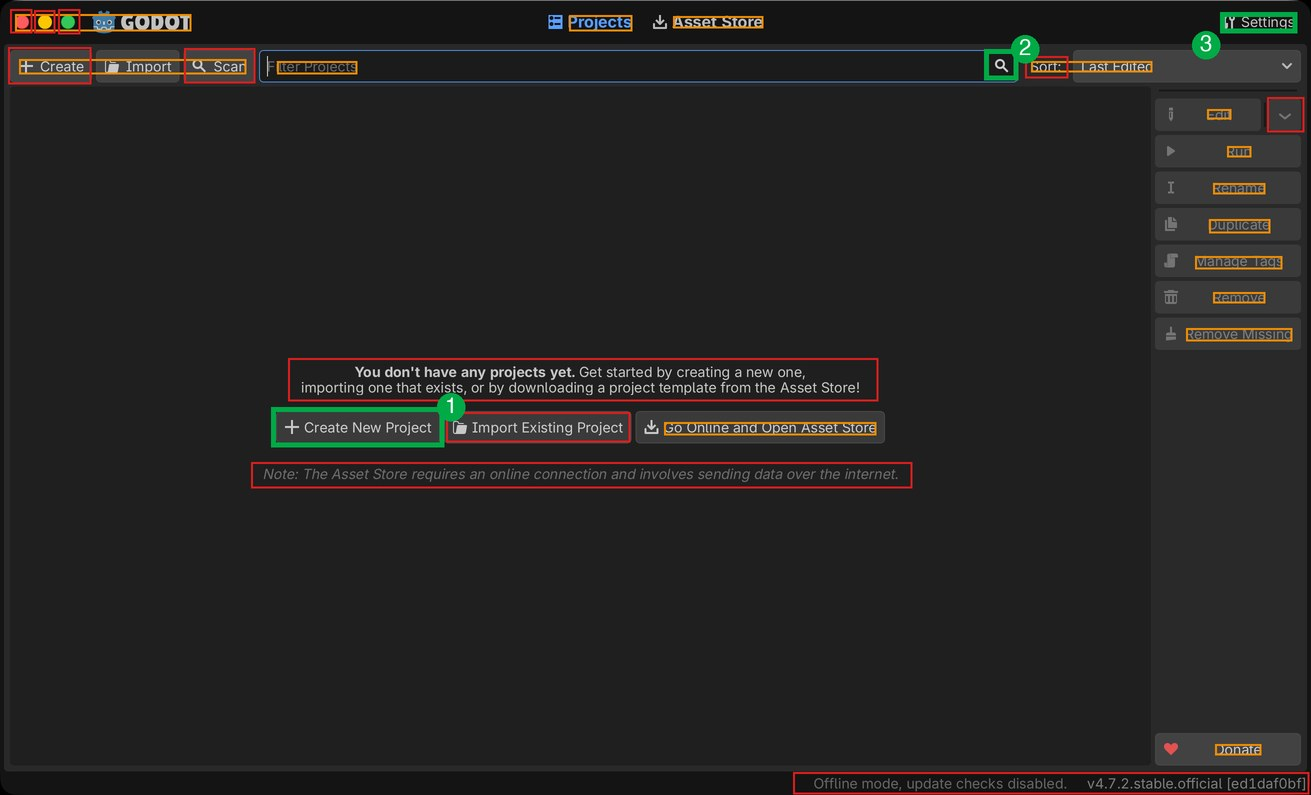
\includegraphics[width=\columnwidth]{fig_godot.jpg}
\caption{A \bench{} screen (Godot's project manager, whose AX tree exposes 10 elements). Reference options: AX (blue), OCR text with no AX element (orange), detector-only boxes (red). Three of its 13 commands, targets in green: (1)~``make a new project'' (icon), (2)~``hit the magnifying glass in the filter box'' (icon), (3)~``open settings'' (OCR). ``run the space shooter project'' is absent: no such project exists.}
\label{fig:example}
\end{figure}

\section{Related Work}
Grounding benchmarks pair a screenshot with an instruction and a target box: ScreenSpot~\cite{seeclick} (mobile, desktop, web), its corrected v2~\cite{osatlas}, ScreenSpot-Pro~\cite{sspro} (high-resolution professional software), OSWorld-G~\cite{jedi} (Ubuntu) and OmniACT~\cite{omniact} (desktop and web scripts). Web agent benchmarks such as Mind2Web~\cite{mind2web} and WebArena~\cite{webarena} expose the DOM, the web analogue of the AX tree, but cover the browser only. Interactive suites such as OSWorld~\cite{osworld} and macOSWorld~\cite{macosworld} score whole tasks; \bench{} isolates the grounding step at larger scale and adds abstention labels. Screen parsers such as OmniParser~\cite{omniparser} build option lists from pixels; \bench{}'s pixels track lets such parsers be compared against the AX tree on the same commands.

\section{Collection}
\textbf{Sandbox capture.} We ran a collector for about 20 hours on each of four EC2 Mac instances (macOS, 1440$\times$900 virtual HiDPI display). Before collection each Mac was seeded with made-up content: contacts, notes, reminders, calendar events and mail for invented people, all with \texttt{@example.com} addresses and 555 phone numbers. Websites were browsed logged out. The collector opened apps and sites, clicked through their controls, and at each step saved the frontmost window composited with any sheets, popovers and the menu bar, the AX tree of the window and menu bar, and window geometry. Images therefore follow the window: small utility windows and dialogs give small images (the smallest is 437$\times$189 pixels), and pop-up menus or page content extending past the window edge are cut off. No command targets an element lying fully outside its image. Each instance was terminated after collection. The full pool has 25,117 screens from 115 apps and sites (40 websites).

\textbf{App-level split.} Apps and sites were split before labelling, stratified by native vs.\ web and by how complete their AX tree is: 80 train, 12 validation, 23 test. No model was trained on the validation apps, so we moved 10 of them into the test set; \bench{} uses these 33 apps only (Table~\ref{tab:stats}), and a model trained on the training split has never seen any of them.

\textbf{Screen selection.} From 9,338 test-app screens we picked screens spread evenly over apps, alternating hard screens (AX-poor or with 3+ icons only a detector finds) with ordinary ones and light with dark mode, and dropping near-duplicates (option-label Jaccard $\geq 0.9$ within an app). Because images follow the window, a sheet or toolbar drawn outside it can be missing from the image while its AX elements remain; we dropped 785 commands whose target region is blank in the image and 62 screens whose open sheet was not captured. 1,350 screens remain.

\textbf{Option lists.} Figure~\ref{fig:example} shows an example. Detector boxes in the shipped lists are named by a deployed captioner (\S5). For each screen we merge three sources into a reference list: AX elements (role, label, context), Apple Vision OCR lines not covered by an AX element, and boxes from a YOLO GUI detector not covered by either. Detector-only boxes are the icons a pixels-only system must find without text.

\textbf{Commands.} Commands were drafted by LLM labelling agents (Claude) that saw the screenshot, with detector-only boxes drawn and numbered, and the option list. Per screen they wrote about 12 commands in two styles, casual (``hit the trash can'') and planner-like (``Open the Sections dropdown''), following a written guide: target only visible elements, refer to icons by look or position, write 2--4 icon commands where a screen has icons, keep 10--15\% absent commands, and add ambiguous and irreversible commands where the screen allows. Each command lists every acceptable target. The author checked a stratified sample of 300 commands (60 per target kind: AX, OCR, icon, menu bar, absent) against the screenshot with the target drawn; all 300 were judged correct (95\% Wilson interval 98.7--100\%). As an independent check, a model from another family (OpenAI, through the Codex CLI) judged every command against the screenshot with all targets drawn. It flagged 735 of 18,768 (3.9\%; 1.2\% on the screens added in this release); we removed the 316 that were wrong and kept the rest, which were false alarms such as small box offsets.

\begin{table}[t]
\caption{\bench{} at a glance.}
\label{tab:stats}
\small
\begin{tabular}{@{}lr@{}}
\toprule
Screens (native / web) & 1,350 (726 / 624) \\
Apps and sites & 33 (22 native, 11 web) \\
Commands & 17,432 \\
\quad target is an AX element & 12,115 \\
\quad target is OCR text with no AX element & 1,236 \\
\quad target is a detector-only icon & 2,086 \\
\quad target is a menu-bar item & 71 \\
\quad target absent (``none'') & 1,924 \\
\quad ambiguous / irreversible & 763 / 94 \\
\bottomrule
\end{tabular}

\vspace{2pt}
\footnotesize Native apps: Audio MIDI Setup, Blender, Cyberduck, Disk Utility, Firefox, Font Book, GIMP, GnuCash, Godot, HandBrake, IINA, Journal, Keka, Krita, MuseScore~4, Music, Notes, Photo Booth, Print Center, Safari, Transmission, Weather. Sites: bbc.com, bestbuy.com, gutenberg.org, irs.gov, khanacademy.org, npr.org, reddit.com, wikihow.com, wikipedia.org, ycombinator.com, youtube.com.
\end{table}

\section{Benchmark}
\textbf{Tracks.} \emph{Pixels only}: the system gets the screenshot and the command; it may use the reference OCR and detector output but not AX (17,361 commands; menu-bar targets are excluded since a closed menu has no pixels). \emph{AX + pixels}: the system also gets the AX tree (all 17,432 commands).

\textbf{Answers.} A system answers with a point, an option id, or ``none''. A point is correct if it falls inside any target box; an option id is correct if it is in the target set. For list-picking models we ship ready-made option lists for both tracks. On the pixels track, 1,057 targets are covered by no OCR line or detector box, so a list model cannot get them right; we score list models over all track commands and count these as errors, so list and point models share one denominator.

\textbf{Metrics.} Element accuracy, overall and by target kind (AX, OCR, icon, menu); abstention accuracy on absent commands and the false-abstain rate on present ones; accuracy on ambiguous and irreversible commands; and, for systems with confidences, calibration (ECE and error rate above 0.9 confidence).

\section{Baselines}
We score list-picking models on the ready-made lists. \emph{Kev-0.8B}~\cite{kev} is a public calibrated decision model built on Qwen3.5-0.8B that returns a probability for each option of a list. \emph{Kev-0.8B-FT} is the same model fine-tuned on 66,497 commands from our 80 training apps, built the same way as \bench{} but with icons from a deployed pipeline (detector, a SigLIP~\cite{siglip} reranker keeping the top 50 icons per command, and a Florence-2~\cite{florence2} captioner trained on AX labels). Two screenshot models answer with points on the pixels track: \emph{UI-Venus-1.5-2B}, trained for GUI grounding, and the general \emph{Qwen3-VL-2B-Instruct}. Their \emph{-FT} versions add a LoRA (rank 64, one epoch) trained on 5,999 training-split screens with 63,230 point answers and 7,151 absent commands, in Venus's prompt format (\texttt{[-1,-1]} for an absent target). Screenshot models are scored on a 3,644-command subset drawn at random within each target kind (21\%); Kev-0.8B-FT scores 64.8\% on this subset against 64.9\% on the full pixels track. In the ready-made lists every detector box is named by the deployed captioner, not by the labelling agents: their icon captions echo the commands (98\% of icon targets share a content word with their command, against 31\% with the deployed captions) and would leak the answer. We release them as annotations only.

\begin{table}[t]
\caption{Element accuracy (\%) on \bench{}. All: every command in the track; columns by target kind (None: absent commands, where only abstaining is right). On the pixels track, list models are charged for the 1,057 targets (8.7\% of AX-kind targets) that no OCR line or detector box covers. $^\dagger$Scored on the 3,644-command subset.}
\label{tab:results}
\small
\setlength{\tabcolsep}{4pt}
\begin{tabular}{@{}llrrrrr@{}}
\toprule
Track & Model & All & AX & OCR & Icon & None \\
\midrule
AX + pixels & Kev-0.8B & 54.7 & 61.1 & 71.8 & 18.0 & 42.4 \\
            & Kev-0.8B-FT & 81.5 & 86.6 & 76.1 & 49.8 & 87.3 \\
\midrule
Pixels only & Kev-0.8B & 46.2 & 51.8 & 52.5 & 20.9 & 34.5 \\
            & Kev-0.8B-FT & 64.9 & 64.4 & 56.6 & 49.8 & 89.6 \\
            & Qwen3-VL-2B$^\dagger$ & 59.9 & 69.9 & 58.9 & 53.5 & 4.7 \\
            & Qwen3-VL-2B-FT$^\dagger$ & 84.2 & 89.5 & 57.4 & 86.8 & 65.7 \\
            & UI-Venus-1.5-2B$^\dagger$ & 81.6 & 89.6 & 64.3 & 87.0 & 37.0 \\
            & UI-Venus-1.5-2B-FT$^\dagger$ & 84.7 & 89.9 & 59.7 & 88.4 & 64.2 \\
\bottomrule
\end{tabular}
\end{table}

\textbf{Results.} The AX tree matters most for list models. With it, Kev-0.8B-FT answers 81.5\% of commands and 86.6\% of AX-kind targets; given only OCR and detector boxes, it answers 64.4\% of the same AX-kind targets, partly because 8.7\% of them are covered by no OCR line or detector box (the pixels-track list ceiling is 93.9\%). Icons are the hard case for list models: although 99.9\% of icon targets are in the pixels list, Kev-0.8B-FT picks the right one half the time, while the screenshot models, which read the pixels directly, hit 87--88\%. The captions that name detector boxes, not the list itself, are the bottleneck.

\emph{Training on Mac data transfers to unseen apps.} Fine-tuning on the training split, which shares no app with \bench{}, lifts Kev by 26.8 points on the AX track and the general Qwen3-VL-2B by 24.3 points on the pixels track, where it overtakes the GUI-specialised UI-Venus (84.2\% against 81.6\%). Most of the gain is abstention: base Qwen3-VL almost never declares a target absent (4.7\%), Venus does so 37.0\% of the time, and both fine-tuned models about 65\%. On public sets the same Qwen3-VL fine-tune also improves (ScreenSpot-v2 macOS 78.2$\to$91.2\%, ScreenSpot-Pro macOS 28.8$\to$54.6\%), while Venus, already trained on such data, loses 3--9 points there (it abstains too often) and gains only on \bench{}. Fine-tuning slightly hurts OCR-only targets (by 2--5 points), which the training split under-represents.

\emph{Abstention and confidence.} The fine-tuned list model abstains correctly on 87--90\% of absent commands with a 7.7\% (AX track) to 12.3\% (pixels track) false-abstain rate. Its confidences are usable: on the AX track 11,245 answers have confidence $\geq 0.9$, and 4.4\% of them are wrong. Accuracy on irreversible (77.7\%) and ambiguous (78.5\%) commands trails the overall figure, and no baseline asks for clarification on ambiguous commands, which they answer like any other.

\section{Availability and Maintenance}
\bench{} is available at \url{https://huggingface.co/datasets/sc3484/macbench} with a datasheet~\cite{datasheets}; the scoring, collection, selection, privacy-scan, build and fine-tuning code is at \url{https://github.com/akhilc08/macbench}. Labels and code are released under CC BY-NC 4.0 (data) and MIT (code); screenshots show Apple's interface and third-party websites, whose rights stay with their owners, and are provided for research use as in prior grounding sets. Releases are versioned; corrections reported through the repository's issue tracker go into point releases with a changelog, and test labels are never retrained on in our own work.

\section{Ethics}
\textbf{Provenance.} All screens come from disposable cloud Macs with made-up personal data; no personal computer or account was used. Websites were visited logged out, without posting or purchasing.

\textbf{Privacy.} Public websites still show real people (news subjects, Wikipedia editors, forum users), and the machines leaked identifiers into some screens. We scanned every string and screenshot for emails, phone numbers, IP addresses, cloud host names, UUIDs, serial numbers, person names and faces (487 of 1,350 screens had at least one hit, most of them public figures' names, authors' bylines or OCR noise), removed screens with private information (profile pages showing emails, a system dialog naming the collection machine, block notices showing IP ranges), and redacted the rest: browser (Safari, Firefox) tab, sidebar and suggestion entries that could point at a private person or place (every search-results tab, user-profile tab and address-bar suggestion, whatever its content, plus street addresses from real-estate listings and handles), volume and snapshot UUIDs, cloud host names, the sandbox account name and public IP addresses. Redacted text is replaced in every field and its box is blurred in the screenshot (4,339 boxes on 593 screens); no command targets a redacted element. Public figures in news content, public business phone numbers and public usernames remain, as on the live sites and in other web screenshot sets.

\textbf{Content.} Screens from an adult forum section the crawler reached were removed.

\textbf{Automated labels.} Commands and icon captions were drafted by an LLM. A 300-command stratified sample was checked by hand and judged fully correct, and a model from another family re-judged every command, but neither rules out rarer errors. Commands may reflect the labelling model's phrasing more than real users'; we release the labelling guide so this can be judged.

\textbf{Misuse.} Better grounding helps both assistive agents and automation that acts without a user's consent. The benchmark contains no credentials, payment flows or personal data, and its irreversible-action labels are meant to help agents ask before acting.

\bibliographystyle{ACM-Reference-Format}
\bibliography{refs}
\end{document}
